\documentclass[12pt]{article}
\usepackage[a4paper, total={6in, 9in}]{geometry}
\usepackage{graphicx}
\graphicspath{ {./images/output/} }
\usepackage{caption}
\usepackage[english]{babel}
\usepackage{titling}
\usepackage{float}
% \usepackage{amsmath}
% \usepackage{minted}
% \usepackage{multicol}
% \usepackage{array}
% \usepackage{setspace}
% \usepackage{placeins}

% \usepackage{lipsum}

\title{Single Phase AC-AC Bidirectional(Full Wave) Voltage Controller with R, RL Load}
\author{}
\date{}

\pagenumbering{gobble}
\begin{document}
\vspace*{\fill}
\begin{center}

    \emph{Heaven's Light is Our Guide} \\
    \textbf{Rajshahi University of Engineering and Technology} \\

    \begin{figure}[H]
        \centering
        
\includegraphics[scale=.34]{images/RUET_logo.png}
        \label{fig:ruet_logo}
    \end{figure}
    \vspace{5mm}

    \textbf{Course Code}\\
    ECE 3206\\
    \vspace{3mm}
    \textbf{Course Title}\\
    Industrial Electronics Sessional

    \vspace{5mm}
    \textbf{Experiment Date:} {January 13, 2025},\\
    \textbf{Submission Date:} {February 10, 2025}\\

    \vspace{5mm}
    \textbf{Lab Report 3: \\
        Study of Thyristor Characteristics R, RL Load}

    \vspace{15mm}

    \begin{tabular}{c|c}
        \textbf{Submitted to} & \textbf{Submitted by} \\
        Md. Faysal Ahamed     & Md. Tajim An Noor     \\
        Lecturer              & Roll: 2010025         \\
        Dept of ECE, Ruet     &                       \\
    \end{tabular}

\end{center}
\vspace*{\fill}


\pagebreak

\tableofcontents

\pagebreak
\pagenumbering{arabic}
\maketitle

\section*{Theory}
\addcontentsline{toc}{section}{Theory}
The Single Phase AC-AC Bidirectional (Full Wave) Voltage Controller is a power electronic circuit that allows control of the output voltage applied to a load by varying the firing angle of thyristors. It is widely used in industrial applications for controlling power delivered to resistive (R) and inductive (RL) loads \cite{rashid2013power}.

\subsection*{Working Principle}
The circuit consists of two thyristors connected in anti-parallel configuration. During the positive half-cycle of the AC input, one thyristor conducts when triggered, while during the negative half-cycle, the other thyristor conducts when triggered. By adjusting the firing angle of the thyristors, the effective RMS voltage applied to the load can be controlled \cite{sen1987principles}.

\subsection*{Behavior with R Load}
For a purely resistive load, the current waveform follows the voltage waveform. The output voltage is a controlled AC waveform, and the power delivered to the load is proportional to the RMS value of the output voltage. The firing angle directly determines the portion of the input voltage waveform applied to the load \cite{mohan2003power}.

\subsection*{Behavior with RL Load}
For an inductive load, the current lags the voltage due to the inductance. This lag affects the conduction period of the thyristors, as the current may continue to flow even after the voltage crosses zero. The output voltage waveform is still controlled by the firing angle, but the current waveform exhibits a phase lag \cite{bose2002modern}.

\subsection*{Applications}
\begin{itemize}
    \item Speed control of AC motors
    \item Light dimming
    \item Heating control
    \item Industrial power regulation
\end{itemize}

The use of MATLAB/Simulink for simulation allows for detailed analysis of the circuit's behavior under different load conditions, enabling optimization for specific applications \cite{mathworks2023simulink}.


\section*{Required Equipments/Software}
\addcontentsline{toc}{section}{Required Equipments/Software}
\begin{itemize}
    \item MATLAB/Simulink
    \item AC Voltage Source
    \item Thyristors (2 in anti-parallel configuration)
    \item Resistive Load (R)
    \item Inductive Load (RL)
    \item Pulse Generator for firing angle control
    \item Measurement Blocks (Voltage and Current)
    \item Scope for waveform visualization
\end{itemize}

\section*{Circuit Diagrams}
\addcontentsline{toc}{section}{Circuit Diagrams}
\begin{figure}[H]
    \centering
    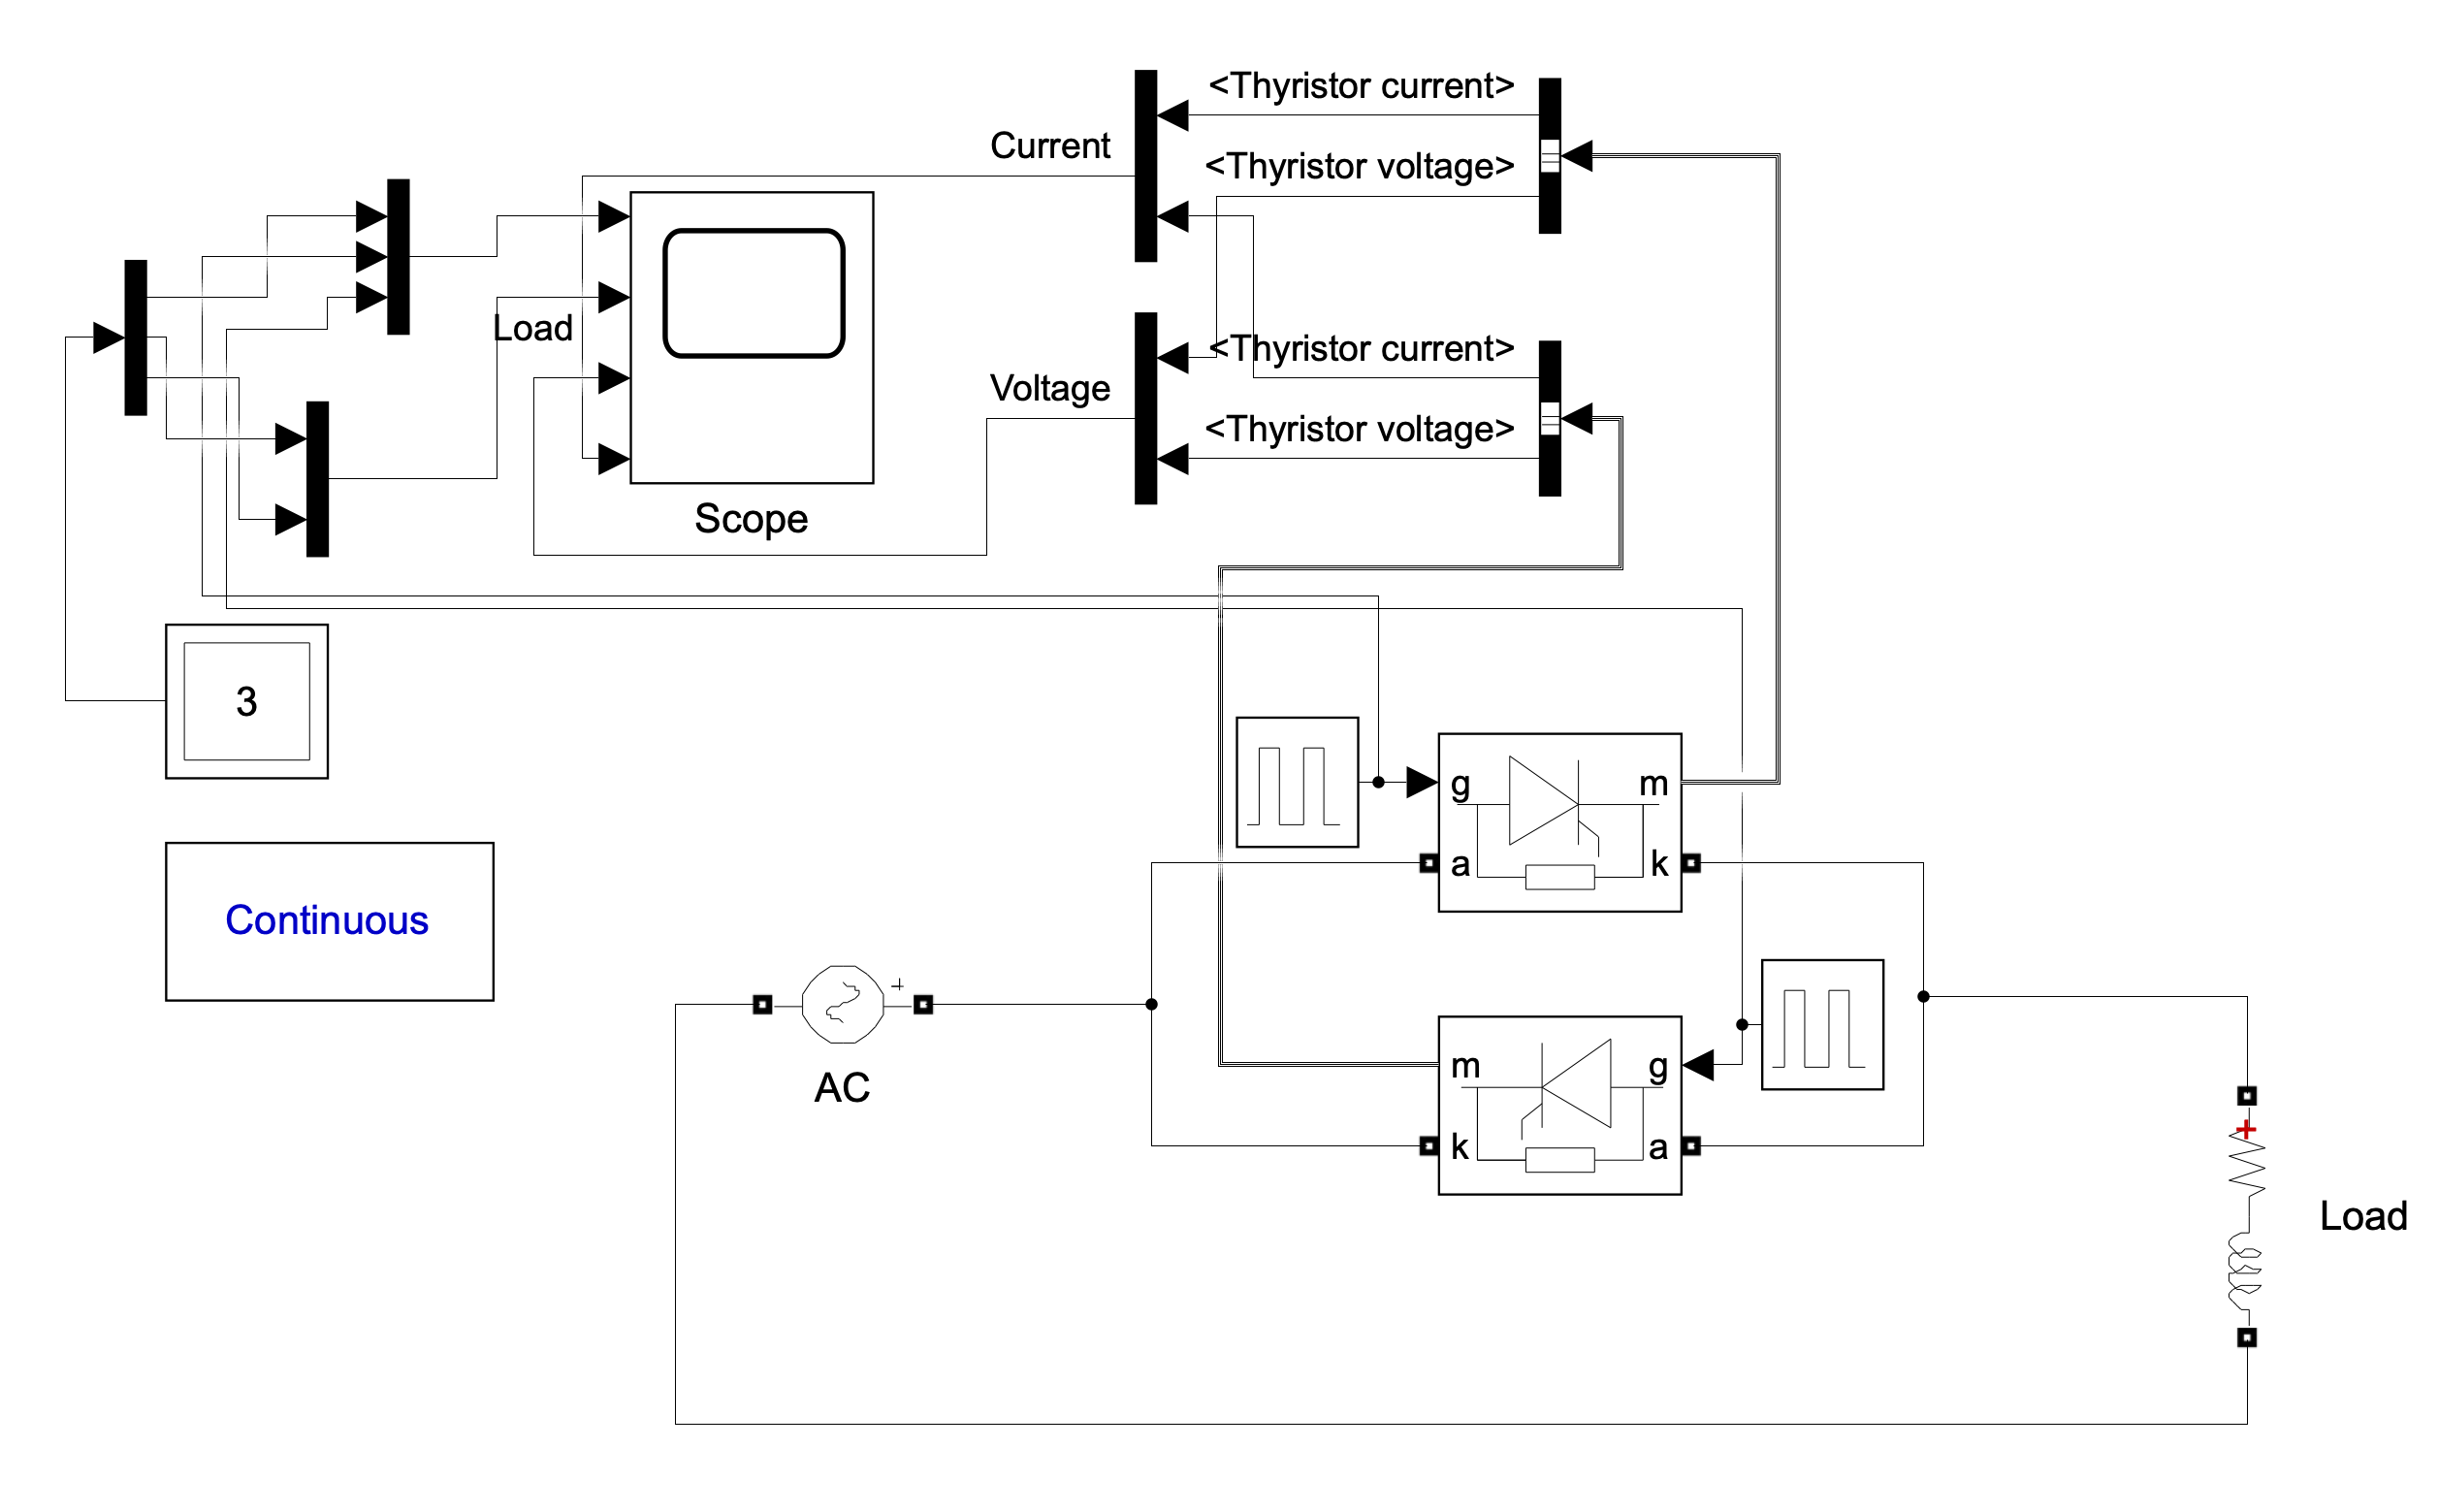
\includegraphics[width=\textwidth]{ckt.png}
    \caption{AC-AC Bidirectional Voltage Controller with R, Rl Load}
\end{figure}

\section*{Observations}
\addcontentsline{toc}{section}{Observations}
\begin{itemize}
    \item For the R load, the output voltage waveform is a controlled AC waveform, with the RMS value depending on the firing angle of the thyristors.
    \item Increasing the firing angle for the R load reduces the effective RMS voltage and power delivered to the load.
    \item For the RL load, the output voltage waveform is controlled by the firing angle, but the current waveform lags due to the inductance.
    \item The lagging current in the RL load causes the thyristors to conduct beyond the zero-crossing of the voltage waveform.
    \item MATLAB/Simulink simulations show the impact of firing angle on the output voltage and current waveforms for both R and RL loads.
    \item The circuit demonstrates effective control of power delivered to the load by varying the firing angle of the thyristors.
    \item The behavior of the circuit under different load conditions highlights the importance of considering load characteristics in power control applications.
\end{itemize}


\subsubsection*{Outputs}
\begin{figure}[H]
    \centering
    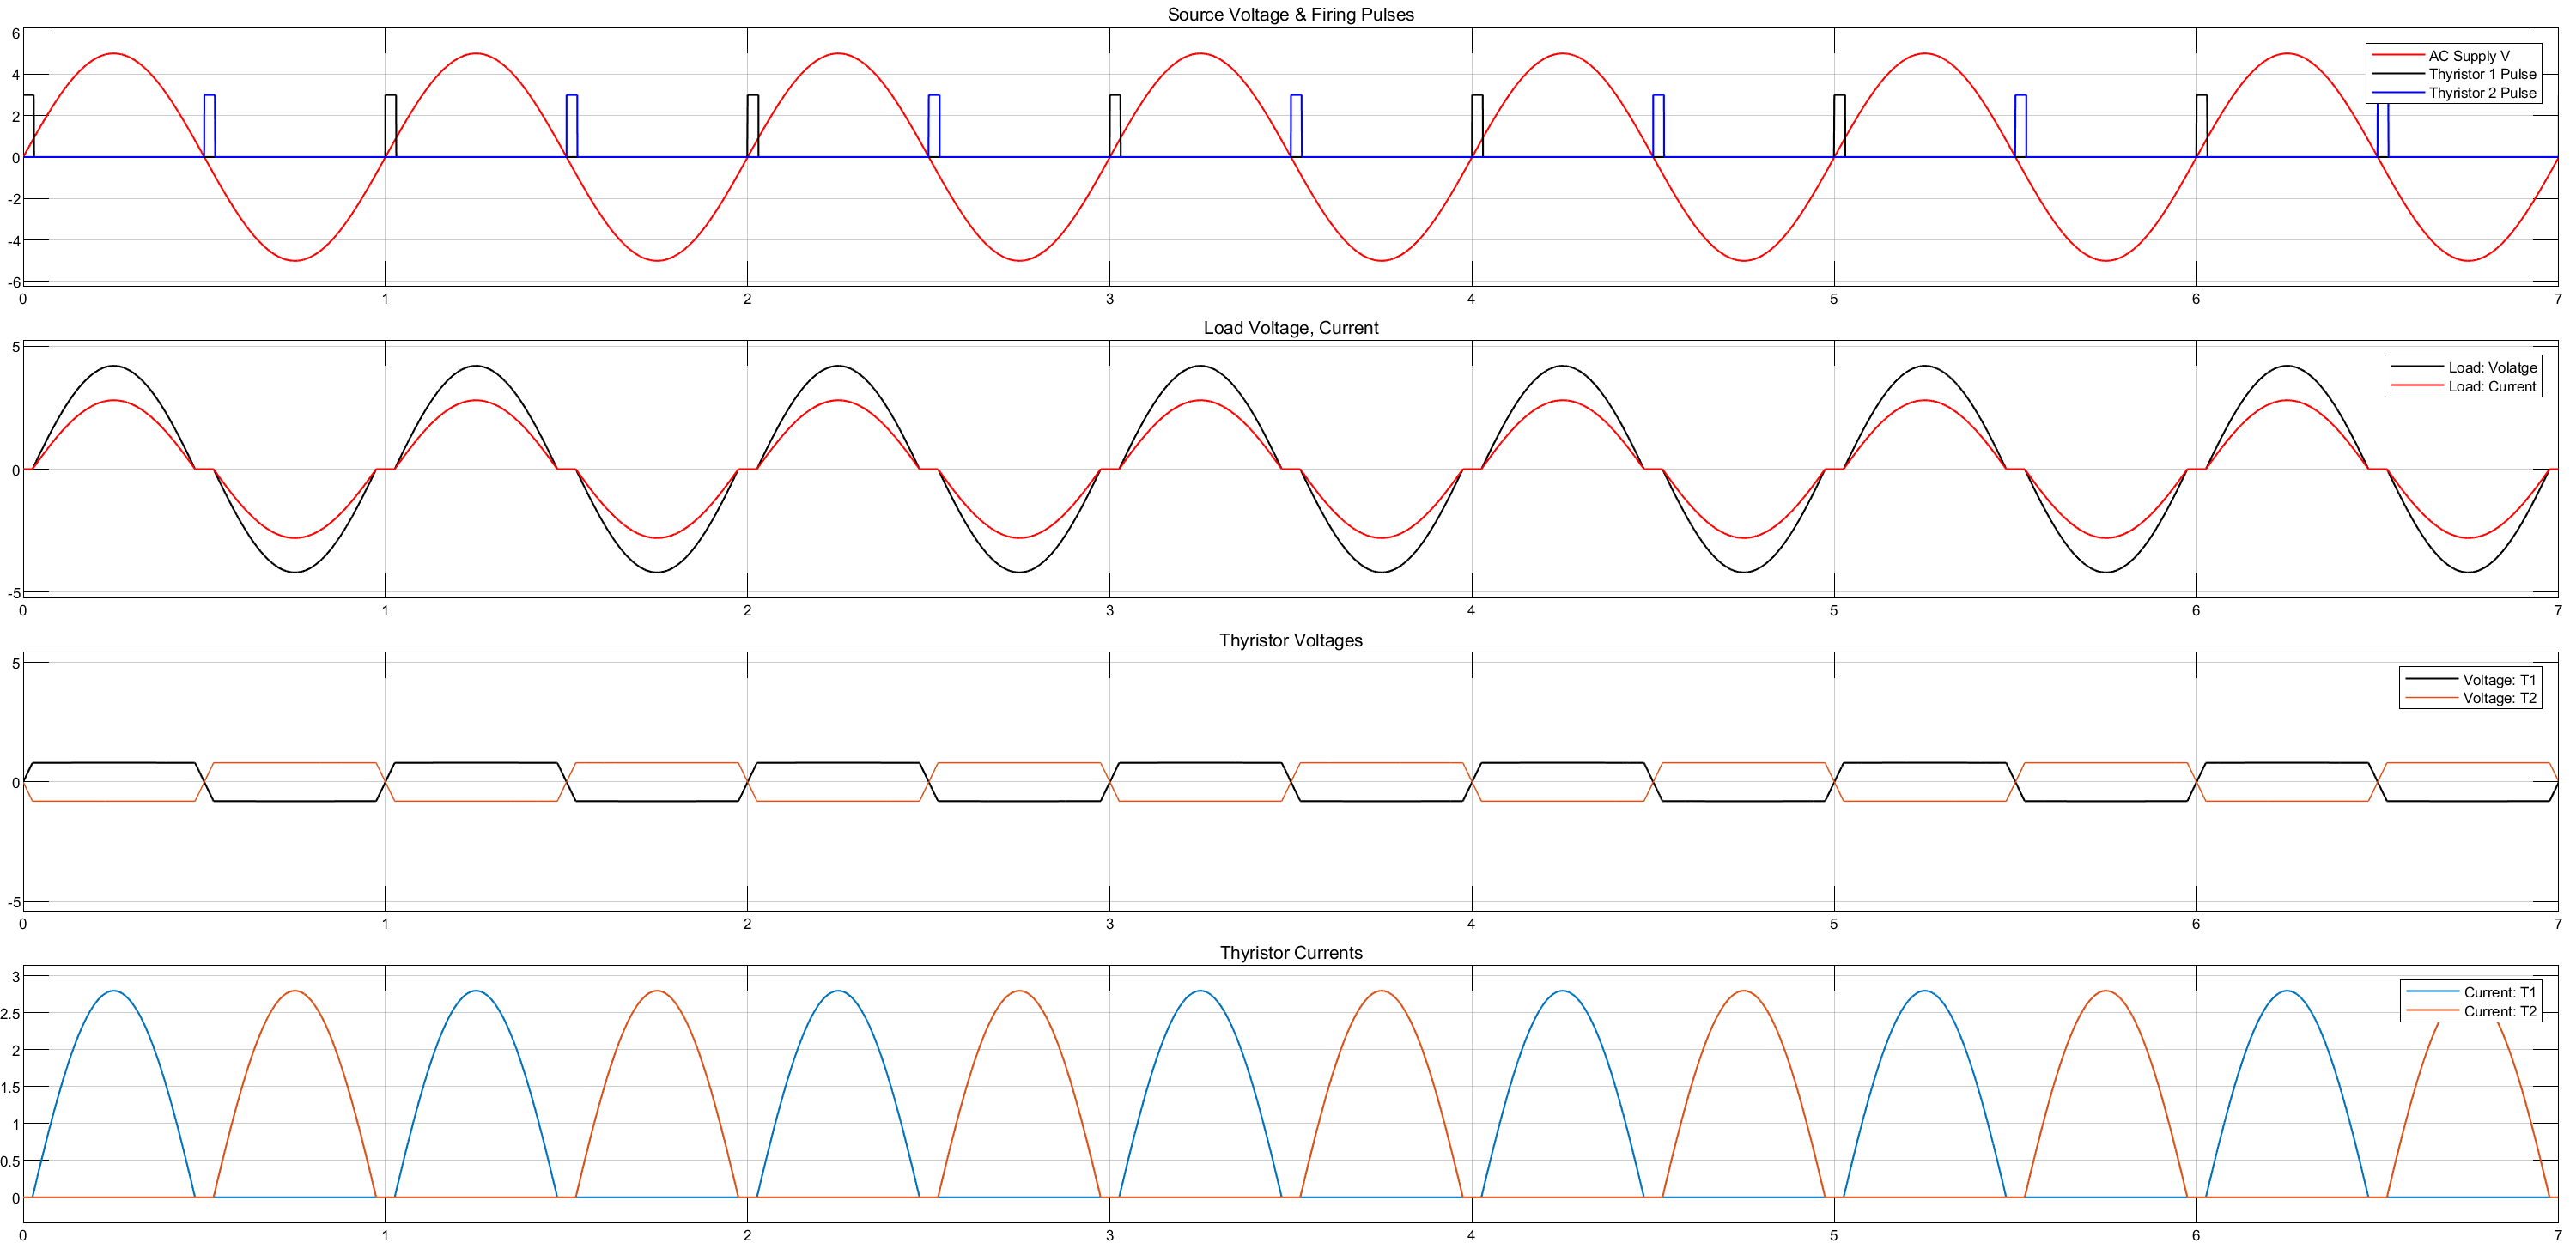
\includegraphics[width=\textwidth]{1Rnd.png}
    \caption{Simulation Output for R Load, Controlled Rectifier, No Delay}
    \label{fig:rControlledNoDelay}
\end{figure}

\begin{figure}[H]
    \centering
    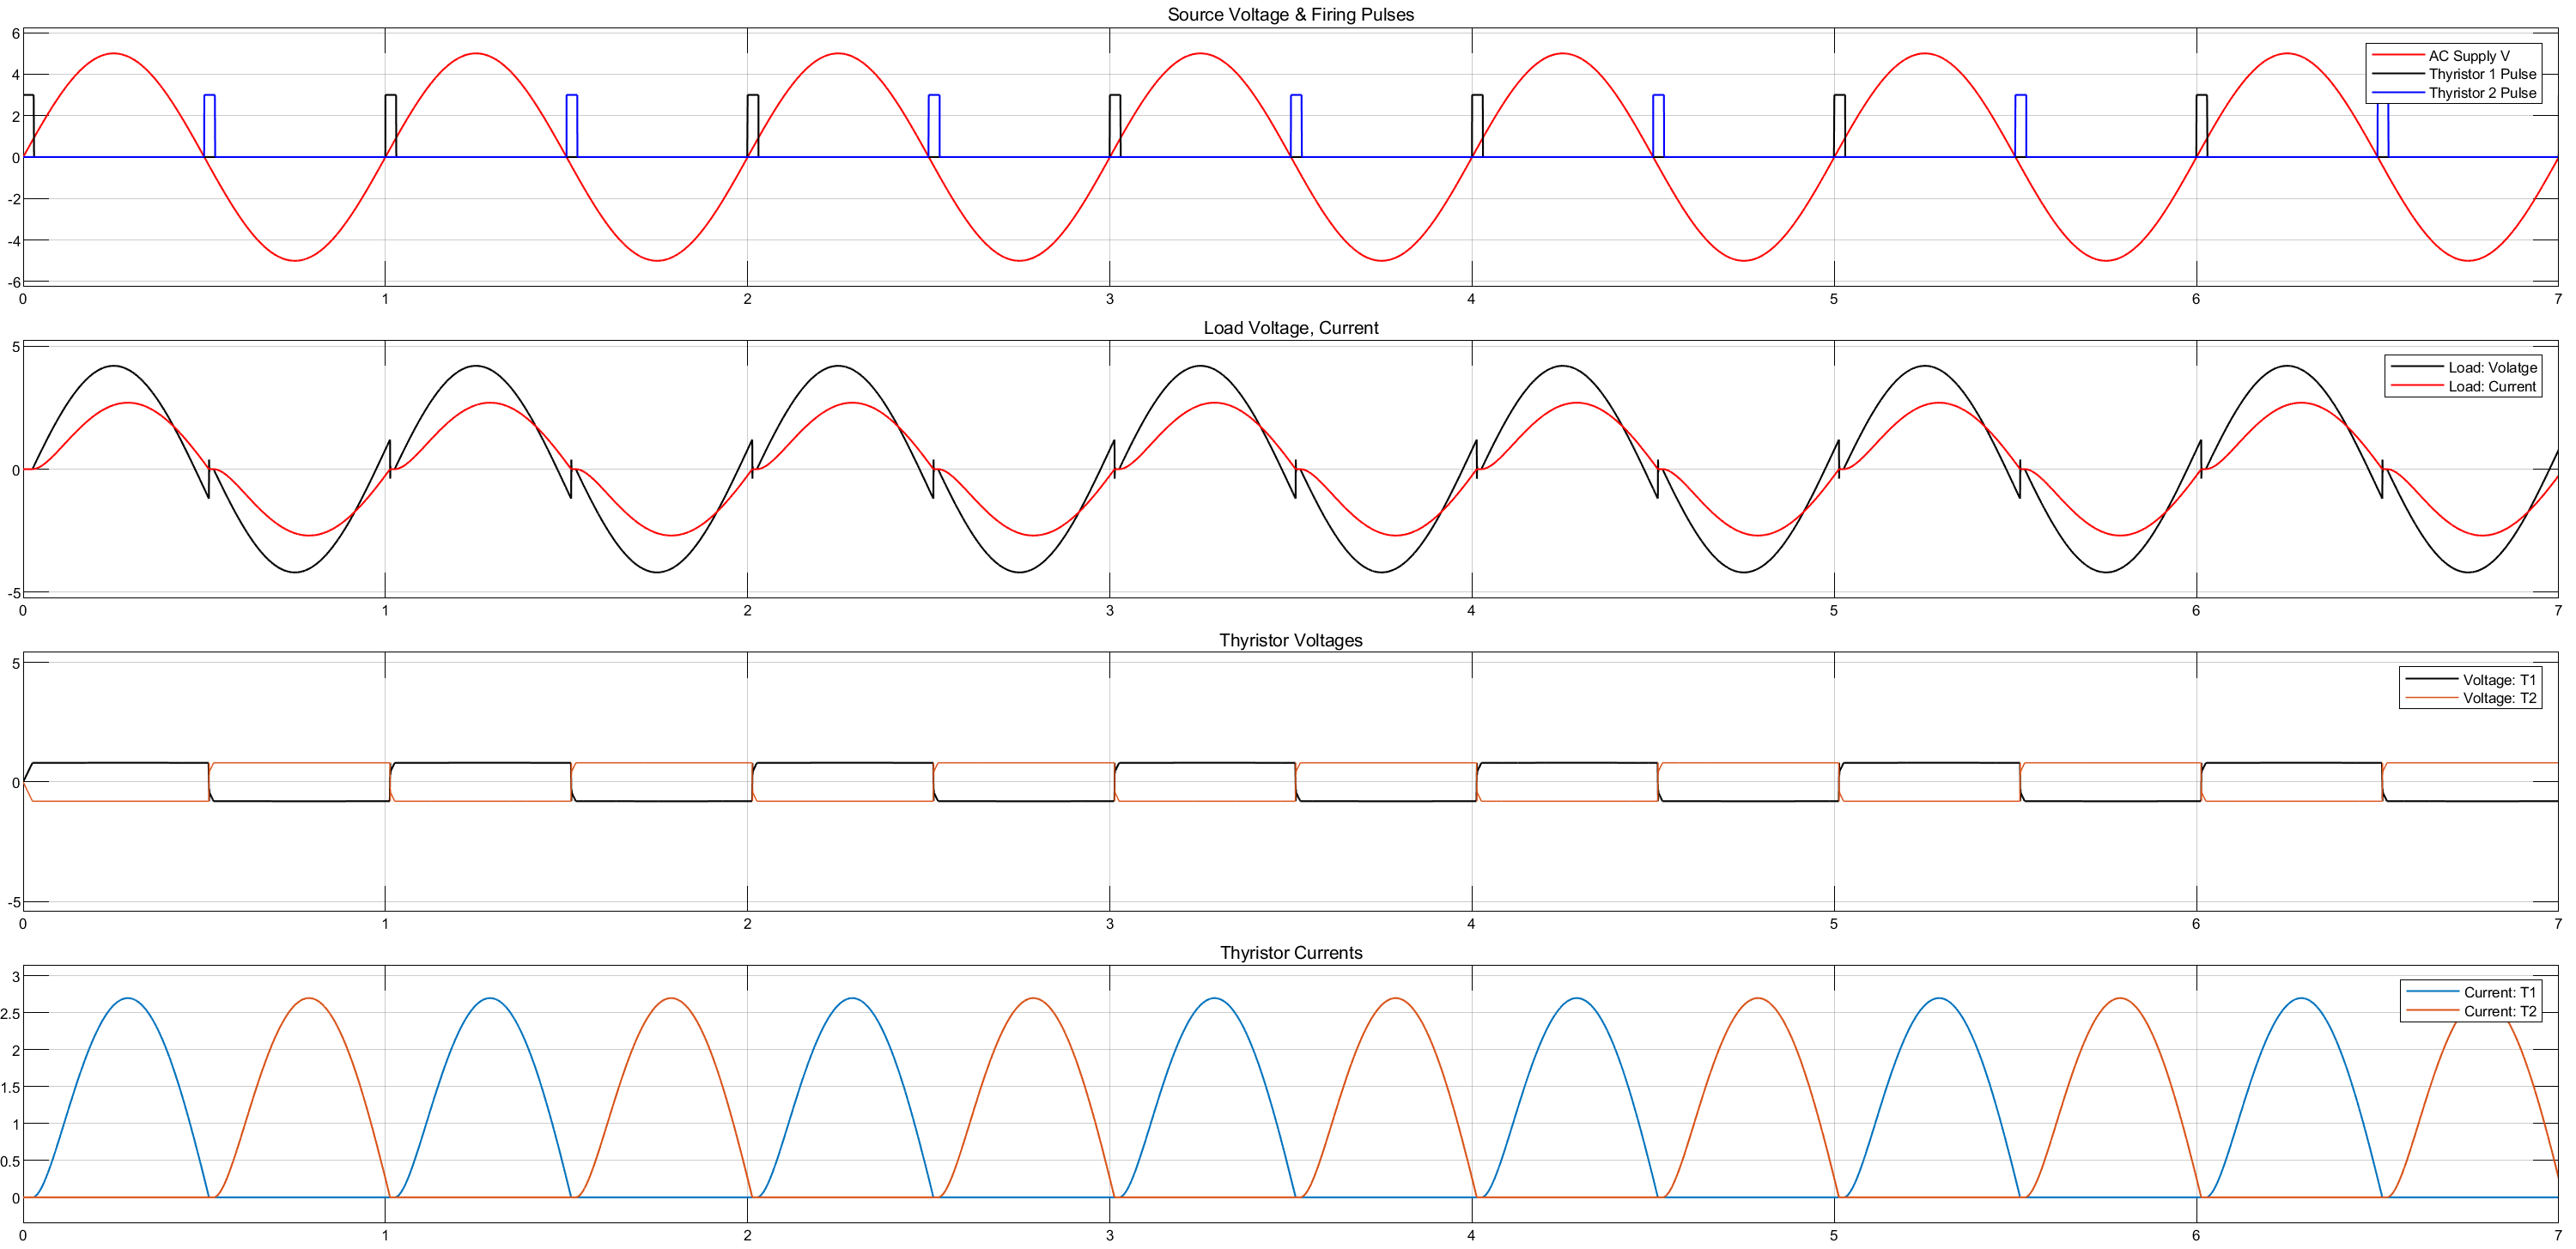
\includegraphics[width=\textwidth]{2RLnd.png}
    \caption{Simulation Output for RL Load, Controlled Rectifier, No Delay}
    \label{fig:rControlledWithDelay}
\end{figure}

\begin{figure}[H]
    \centering
    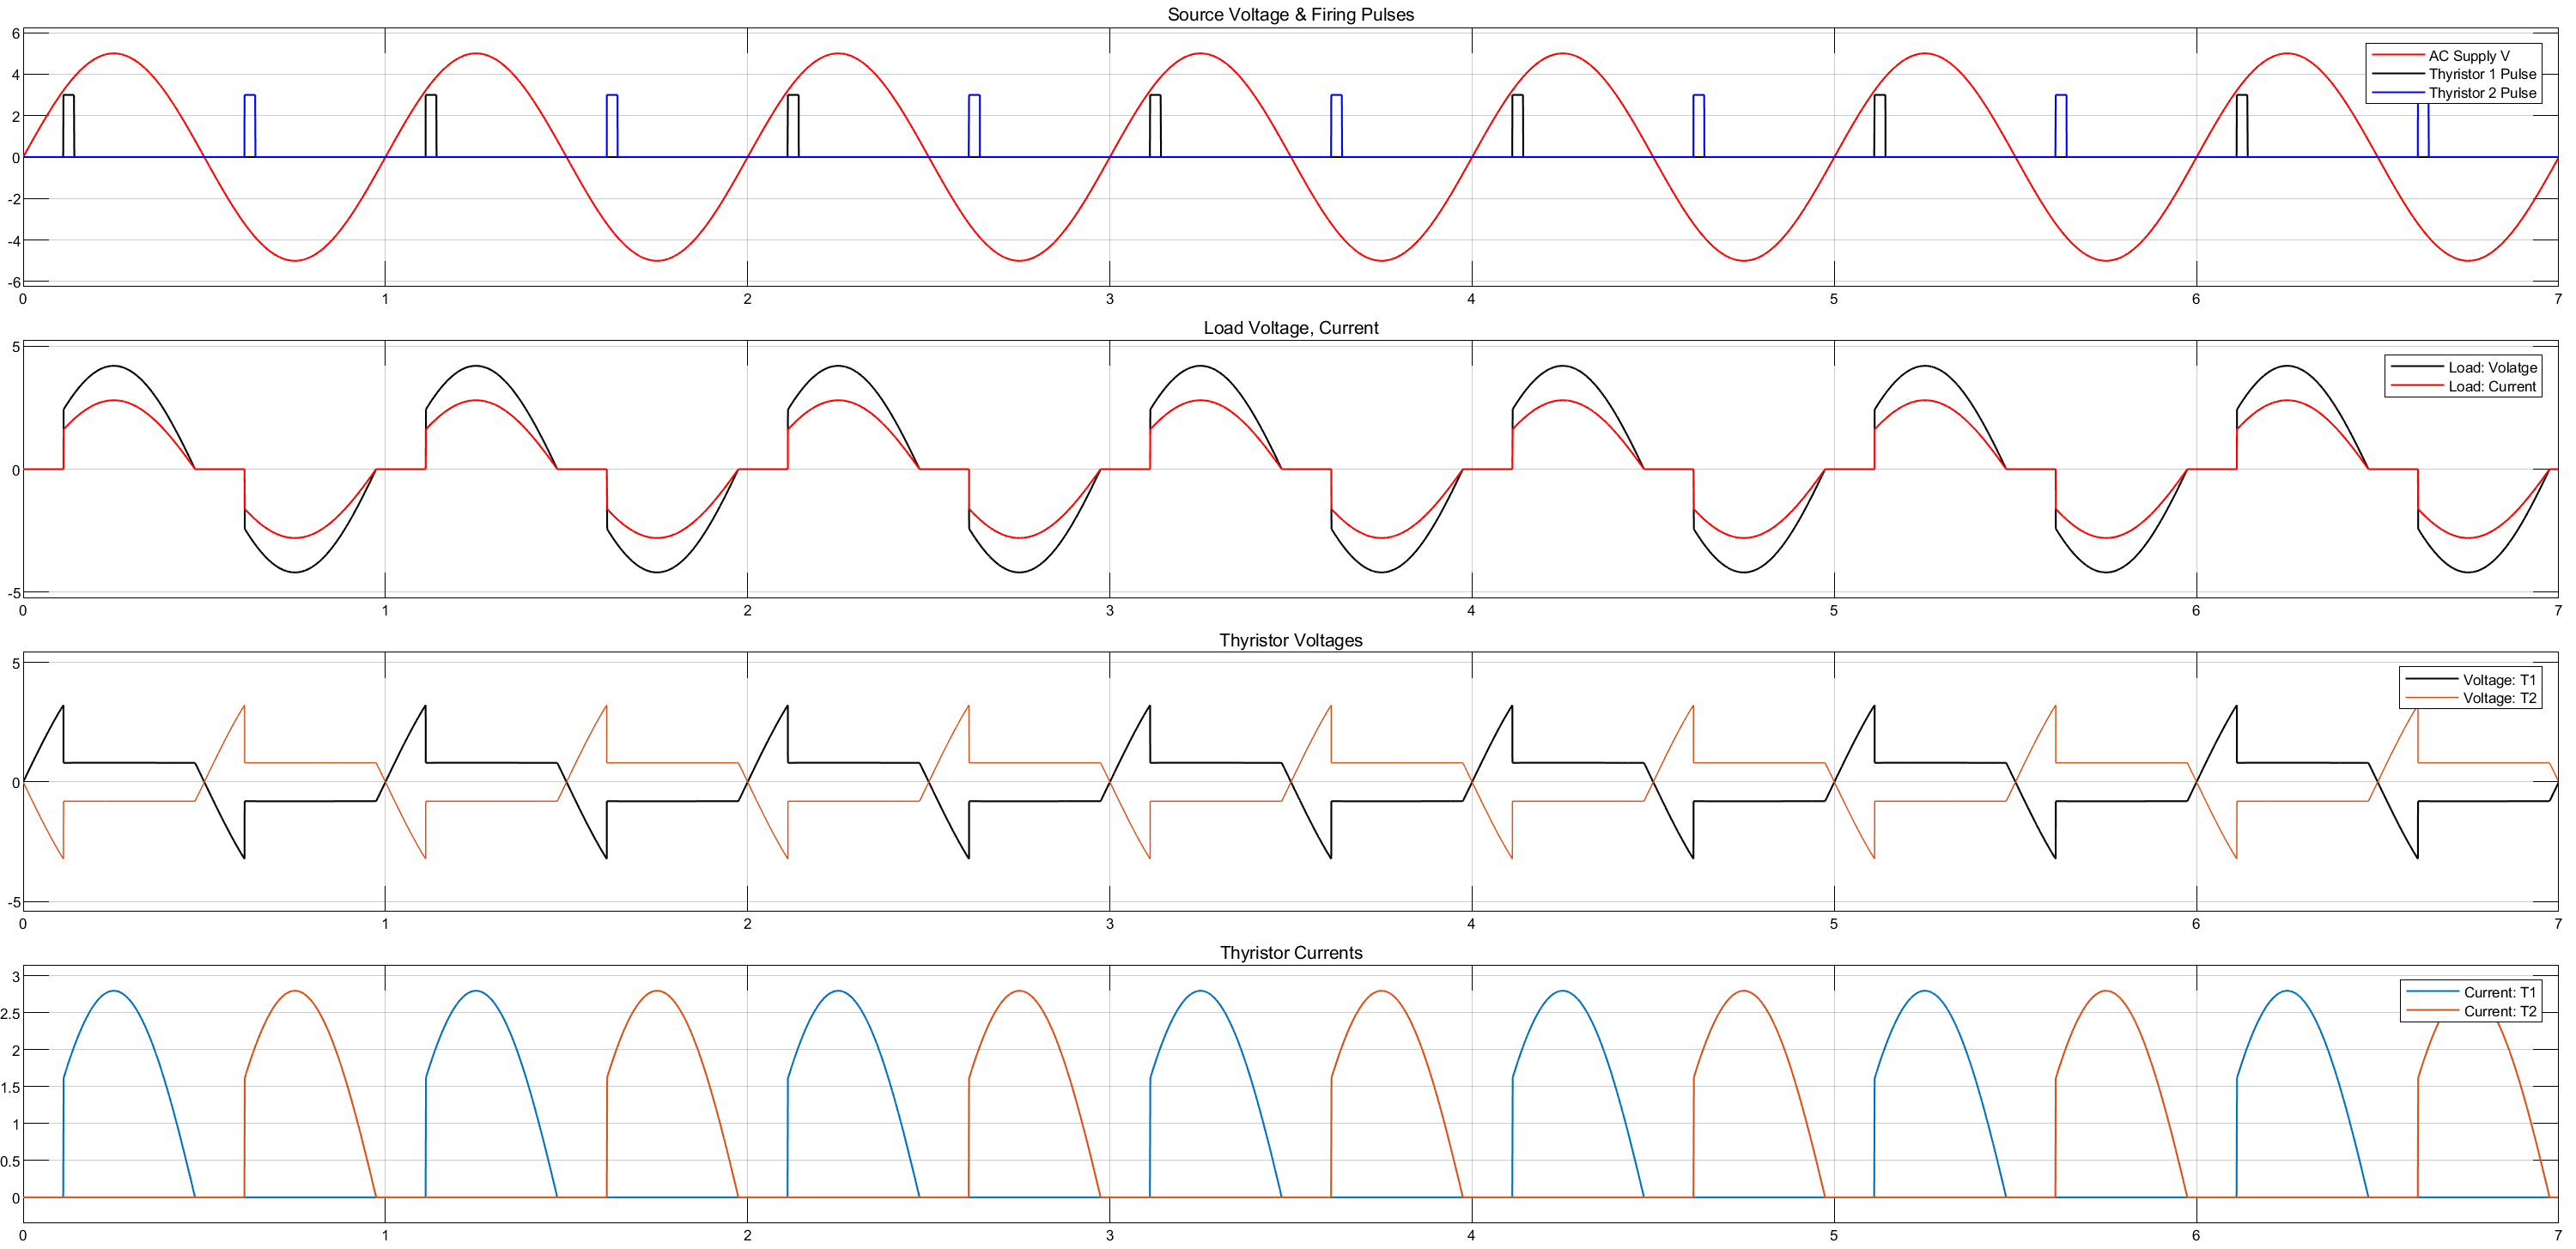
\includegraphics[width=\textwidth]{3Rd.png}
    \caption{Simulation Output for R Load, AC-AC Bidirectional Voltage Controller}
    \label{fig:rLoad}
\end{figure}

\begin{figure}[H]
    \centering
    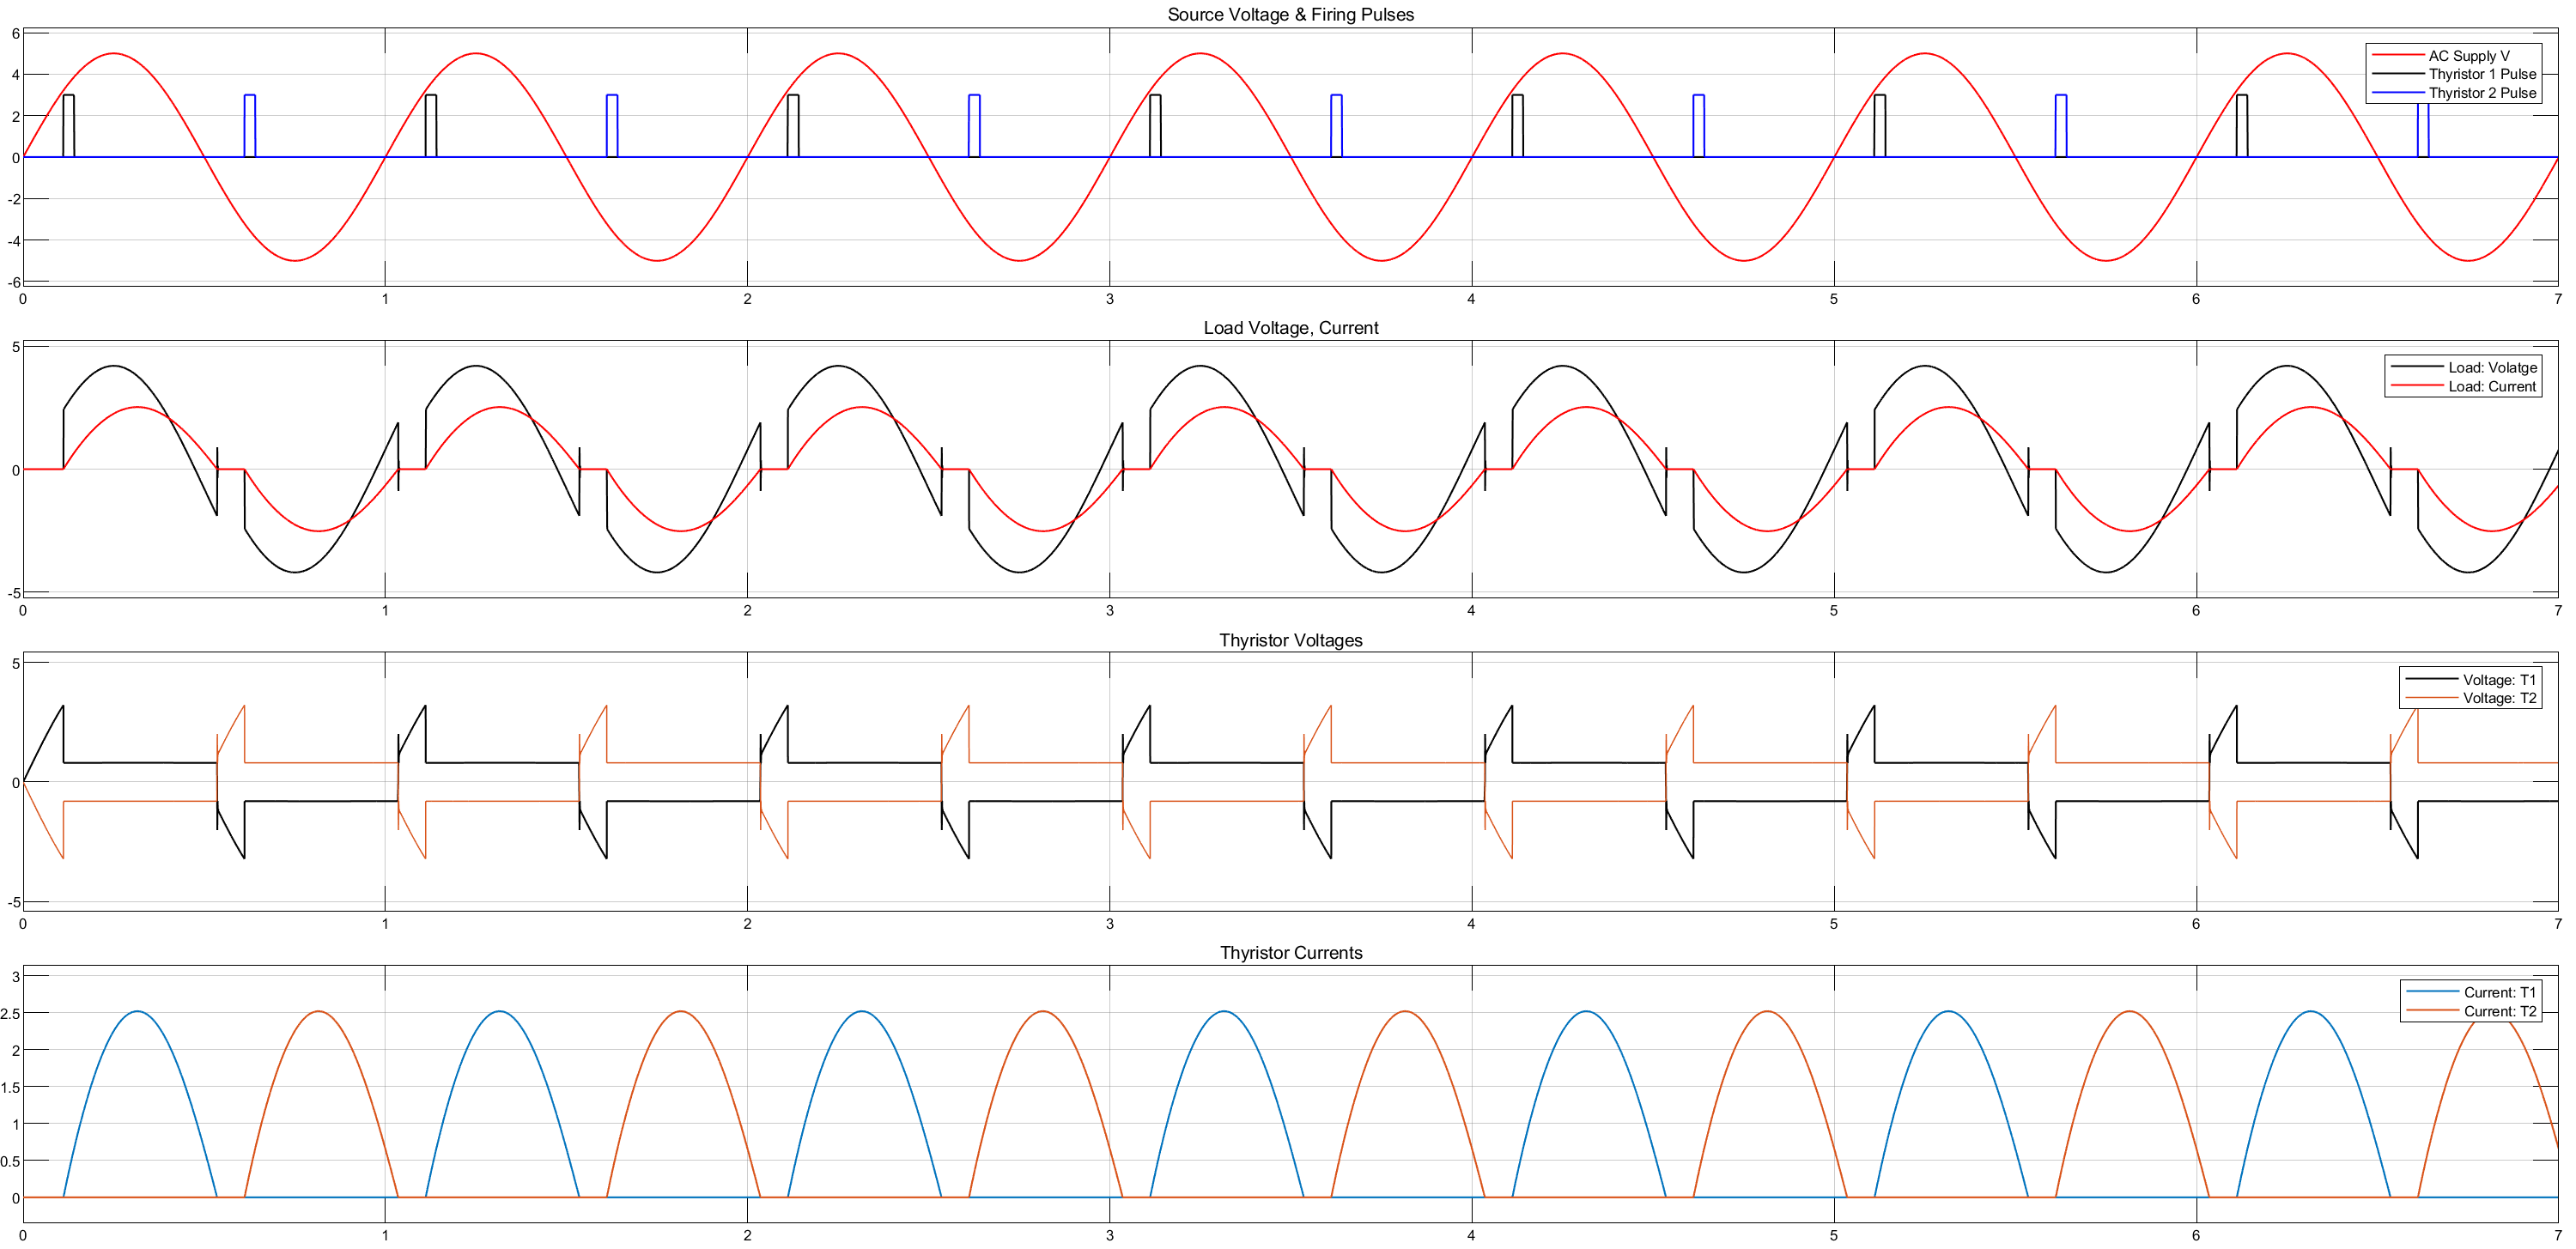
\includegraphics[width=\textwidth]{4RLd.png}
    \caption{Simulation Output for RL Load, AC-AC Bidirectional Voltage Controller}
    \label{fig:rlLoad}
\end{figure}


\section*{Discussion}
\addcontentsline{toc}{section}{Discussion}
The Single Phase AC-AC Bidirectional (Full Wave) Voltage Controller is an essential circuit for controlling power delivered to various types of loads. Through MATLAB/Simulink simulations, we observed the impact of firing angle on the output voltage and current waveforms for both resistive (R) and inductive (RL) loads. The results highlight the importance of precise firing angle control in achieving desired power regulation. For R loads, the output voltage waveform closely follows the input waveform, while for RL loads, the current lags the voltage due to inductance, affecting the conduction period of the thyristors.

\section*{Conclusion}
\addcontentsline{toc}{section}{Conclusion}
The study of the Single Phase AC-AC Bidirectional Voltage Controller with R and RL loads demonstrates its effectiveness in controlling power delivery by varying the firing angle of thyristors. The circuit's behavior under different load conditions emphasizes the need to consider load characteristics in power control applications. MATLAB/Simulink simulations provide valuable insights into the circuit's performance, enabling optimization for industrial applications such as motor speed control, heating, and lighting.

\bibliographystyle{IEEEtran}
\renewcommand{\bibname}{References}
\addcontentsline{toc}{section}{References}
\bibliography{ref}

\end{document}
